\section{Object diffusion mini-protocol}%
\label{sec:object-diffusion-protocol}

This section presents a generic object diffusion mini-protocol.
Heavily inspired by Tx-Submission, we hope to use it for certificate and vote diffusion.
This protocol aims are synchronising a data base of objects (e.g., for Tx-Submission, their mempool) between peers:
%
\begin{itemize}
\item
  Clients and server maintain the knowledge of a queue of objects of which the server has knowledge and the client presumably does not.
  Importantly, the queue is of bounded size, and the maximal size is a hardcoded parameter of the
  implementation.
  The objects are represented by {\em identifiers}, typically orders of magnitude smaller than the objects themselves.

\item
  Clients can ask their servers to provide them with an ordered list of the {\em next} objects that they wish to diffuse.
  The notion of order---and therefore of which objects are {\em next}---is internal to each server; it might for instance be the order in which they themselves got aware of the objects in question.

\item
  Clients can then, given an object identifier, request the corresponding object to the server.
  This is not mandatory, and, if several servers propose to diffuse the same objects, the peer might decide to download only from a subset of them.
  The strategy may vary depending on the objects, how promptly the client wants to get them, and how important it is for them not to miss one.

\item
  When requesting the next batch of object identifiers, the client informs the server that they are not interested in some of the objects anymore, possibly because they have acquired them from this server or another one.
  They do that by {\em acknowledging} a number of identifiers from the beginning of the queue.
  They must, in doing so, ensure that the queue remains under the maximal allowed size.
\end{itemize}

\Cref{fig:object-diffusion-state-machine} gives a graphical representation of the state machine of the proposed mini-protocol, while \cref{fig:object-diffusion-state-agencies} provides a table with the states' agencies.
The coming subsections give more details on the mini-protocol.

\definecolor{mygreen}{rgb}{0.109804,0.698039,0.341176}
\definecolor{myblue}{rgb}{0.360784,0.423529,255}

\usetikzlibrary{automata, positioning, arrows}
\usetikzlibrary{arrows,calc,matrix,shapes}

\tikzset{
    state/.style={
           rectangle,
           rounded corners,
           draw=black, very thick,
           minimum height=2em,
           inner sep=2pt,
           text centered,
           },
}

\newcommand{\header}[1]{\textbf{#1}}

\newcommand{\state}[1]{\texttt{#1}}
\newcommand{\trans}[1]{\texttt{#1}}
\newcommand{\msg}[1]{\textbf{\texttt{#1}}}

\newcommand{\Client}{\textcolor{mygreen}{\textbf{Client}}}
\newcommand{\Server}{\textcolor{myblue}{\textbf{Server}}}

\newcommand{\StInit}             {\state{StInit}}
\newcommand{\StIdle}{\state{StIdle}}
\newcommand{\StBusy}{\state{StBusy}}
\newcommand{\StDone}{\state{StDone}}
\newcommand{\StObjIdsBlocking}    {\state{StObjIdsBlocking}}
\newcommand{\StObjIdsNonBlocking} {\state{StObjIdsNonBlocking}}
\newcommand{\StObjs}              {\state{StObjs}}

\newcommand{\MsgInit}            {\msg{MsgInit}}
\newcommand{\MsgRequestObjIdsNB}  {\msg{MsgRequestObjIdsNonBlocking}}
\newcommand{\MsgRequestObjIdsB}   {\msg{MsgRequestObjIdsBlocking}}
\newcommand{\MsgReplyObjIds}      {\msg{MsgReplyObjIds}}
\newcommand{\MsgRequestObjs}      {\msg{MsgRequestObjs}}
\newcommand{\MsgReplyObjs}        {\msg{MsgReplyObjs}}
\newcommand{\MsgDone}{\msg{MsgDone}}

\begin{figure}[h]
  \begin{center}
    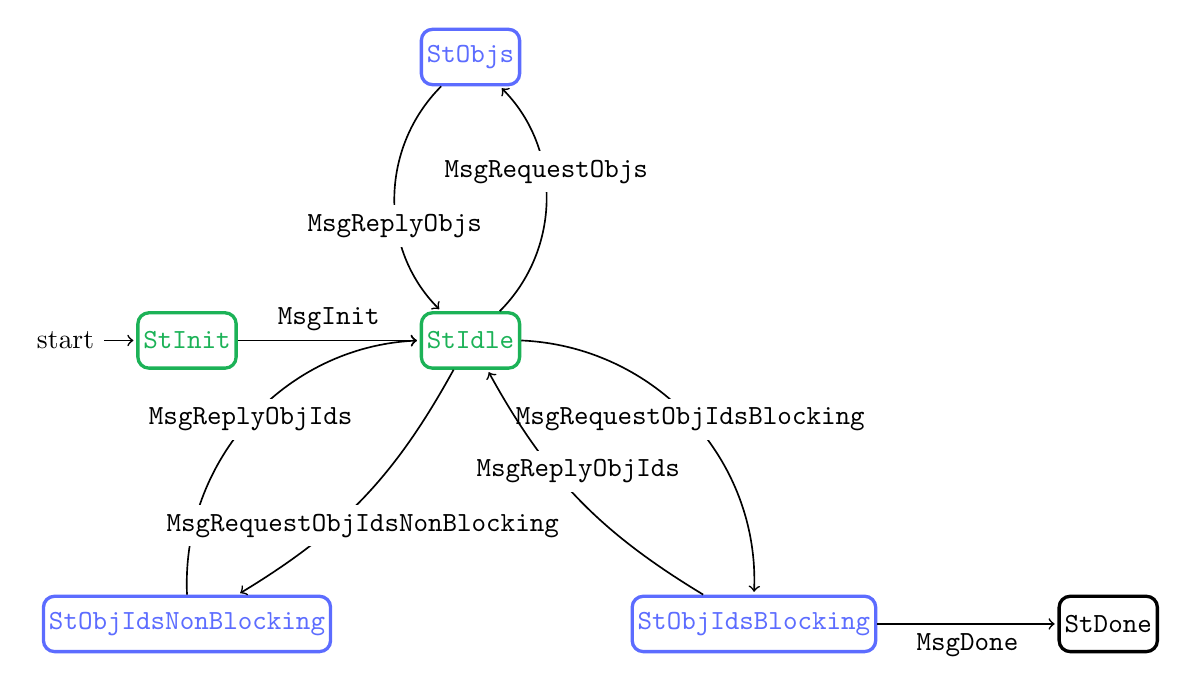
\begin{tikzpicture}[->,shorten >=1pt,auto,node distance=4.5cm, semithick, scale=0.9]
      \tikzstyle{every state}=[fill=red,draw=none,text=white]
      \node[state, mygreen, initial] (I) at (-4,  0) {\StInit};
      \node[state, mygreen]           (A) at ( 0,  0) {\StIdle};
      \node[state]                   (B) at ( 9, -4) {\StDone};
      \node[state, myblue]          (C) at ( 4, -4) {\StObjIdsBlocking};
      \node[state, myblue]          (D) at (-4, -4) {\StObjIdsNonBlocking};
      \node[state, myblue]          (E) at ( 0,  4) {\StObjs};
      \draw (I)  edge[above]                    node[above]{\MsgInit}                                                 (A);
      \draw (C)  edge[above]                    node[below]{\MsgDone}                                                 (B);
      \draw (A)  edge[left, bend left=45]       node[fill = white, anchor = center]{\MsgRequestObjIdsB}               (C);
      \draw (C)  edge[right, bend left=15]      node[fill = white, anchor = center, above = 2pt]{\MsgReplyObjIds}     (A);
      \draw (D)  edge[right, bend left=45]      node[fill = white, anchor = center]{\MsgReplyObjIds}                  (A);
      \draw (A)  edge[right, bend left=15]      node[fill = white, anchor = center, below = 2pt]{\MsgRequestObjIdsNB} (D);
      \draw (A)  edge[left, bend right=45]      node[fill = white, anchor = center, above = 2pt]{\MsgRequestObjs}     (E);
      \draw (E)  edge[right,bend right=45]      node[fill = white, anchor = center, below = 2pt]{\MsgReplyObjs}       (A);
    \end{tikzpicture}
  \end{center}
  \caption{Object diffusion state machine}%
  \label{fig:object-diffusion-state-machine}
\end{figure}

\begin{figure}[h]
  \begin{center}
    \begin{tabular}{l|l}
      \header{state}       & \header{agency} \\\hline
      \StInit              & \Client \\
      \StIdle              & \Client \\
      \StObjIdsBlocking    & \Server \\
      \StObjIdsNonBlocking & \Server \\
      \StObjs              & \Server \\
    \end{tabular}
  \end{center}
  \caption{Object diffusion state agencies}%
  \label{fig:object-diffusion-state-agencies}
\end{figure}

\subsection{Parameters}

This subsection describes the parameters of this generic protocol.
They are notions that need to be made concrete for each implementation of the protocol.

\newcommand\argfont[1]{\textbf{\texttt{\textit{#1}}}}

\begin{description}
\item [\argfont{object}] The abstract type of objects diffused by the protocol.
\item [\argfont{id}] Identifier that uniquely identifies an object.
\item [\argfont{objectIds}] An opaque type returned by the server when asked for object ids.
  It is not explicitely a list of $\argfont{id}$, because the server may want to add metadata to the ids, and/or run a compression scheme to limit the size of its response.
\item [\argfont{responseToIds}] A function with type $\argfont{objectIds} \rightarrow [\argfont{id}]$.
\item [\argfont{initialPayload}] An abstract payload that helps initialise the state of the server.
  For instance, a slot number before which the client does not care about the objects.
  \niols{eg. for Cert-Diffusion it would be a round number, for Vote-Diffusion it would be unit}
\end{description}

\subsection{Protocol messages}

\begin{description}
\item [\MsgInit{} {\((\argfont{initialPayload})\)}]
      Initial message of the protocol, with its payload.

\item [\MsgRequestObjIdsNB{} {$(\argfont{ack},\argfont{req})$}]
      The client asks for up to \argfont{req} new object ids and acknowledges \argfont{ack} old ids.
      The server immediately replies (possibly with an empty list).

\item [\MsgRequestObjIdsB{} {$(\argfont{ack},\argfont{req})$}]
      The client asks for up to \argfont{req} new object ids and acknowledges \argfont{ack} old ids.
      The server will block until new objects are available.

\item [\MsgReplyObjIds{} {$(\argfont{objectIds})$}]
      The server replies with the ids of its available objects.
      In the blocking case, the reply is guaranteed to contain enough information to build at least one object id with \argfont{responseToIds}.
      In the non-blocking case, the reply may not contain any actual data.

\item [\MsgRequestObjs{} {$([\argfont{id}])$}]
      The client requests objects by sending a list of object ids.
      The total size of the corresponding objects MUST not be bigger than the size limit in bytes.
      \niols{Or maybe a bit less; should we take into account the size of the boilerplate?}

\item [\MsgReplyObjs{} {$([\argfont{object}])$}]
      The server replies with the list of all the objects that were requested.
      \niols{Maybe sometimes it is not possible to derive an \argfont{id} from an \argfont{object}? eg. with certificates that could be just a hash? In those cases, wouldn't we want to return a list of pairs \((\argfont{id}, \argfont{object})\)?}

\item [\MsgDone]
      The server terminates the mini protocol.
\end{description}

\Cref{table:object-diffusion-transitions} presents the state transitions and the associated messages.

\begin{table}[h]
  \begin{center}
    \begin{tabular}{l|l|l|l}
      \header{from state}  & \header{message}    & \header{to state}    \\\hline
      \StInit              & \MsgInit            & \StIdle              \\
      \StIdle              & \MsgRequestObjIdsNB & \StObjIdsNonBlocking \\
      \StIdle              & \MsgRequestObjIdsB  & \StObjIdsBlocking    \\
      \StObjIdsNonBlocking & \MsgReplyObjIds     & \StIdle              \\
      \StObjIdsBlocking    & \MsgReplyObjIds     & \StIdle              \\
      \StIdle              & \MsgRequestObjs     & \StObjs              \\
      \StObjs              & \MsgReplyObjs       & \StIdle              \\
      \StIdle              & \MsgDone            & \StDone              \\
    \end{tabular}
  \end{center}
  \caption{Object diffusion mini-protocol state transitions}
  \label{table:object-diffusion-transitions}
\end{table}

\subsection{Size limits and timeouts per state}
\niols{FIXME}

\Cref{table:object-diffusion-size-limits} specifies how many bytes can be sent in a given state; indirectly, this limits the payload size of each message.
If a space limit is violated, the connection SHOULD be torn down.


\Cref{table:object-diffusion-timeouts} specifies message timeouts in a given state.
If a timeout is violated, the connection SHOULD be torn down.

\begin{table}[h]
  \begin{center}
    \begin{tabular}{l|r}
      \header{state}      & \header{size limit in bytes} \\\hline
      \StInit             & \texttt{5760} \\
      \StIdle             & \texttt{5760} \\
      \StObjIdsBlocking    & \texttt{2500000} \\
      \StObjIdsNonBlocking & \texttt{2500000} \\
      \StObjs              & \texttt{2500000} \\
    \end{tabular}
    \caption{Size limits per state}
    \label{table:object-diffusion-size-limits}
  \end{center}
\end{table}

\begin{table}[h]
  \begin{center}
    \begin{tabular}{l|r}
      \header{state}      & \header{timeout} \\\hline
      \StInit             & - \\
      \StIdle             & - \\
      \StObjIdsBlocking    & - \\
      \StObjIdsNonBlocking & \texttt{10}s \\
      \StObjs              & \texttt{10}s \\
    \end{tabular}
    \caption{Timeouts per state}
    \label{table:object-diffusion-timeouts}
  \end{center}
\end{table}

\subsection{CDDL encoding specification}
\label{object-diffusion-cddl}
\niols{FIXME, but maybe it doesn't make sense at all if it is just wildly
  generalised.}

\lstset{
  xleftmargin=2pt,
  stepnumber=1,
  belowcaptionskip=\bigskipamount,
  captionpos=b,
  escapeinside={*'}{'*},
  language=haskell,
  tabsize=2,
  emphstyle={\bf},
  commentstyle=\it,
  stringstyle=\mdseries\rmfamily,
  showspaces=false,
  keywordstyle=\bfseries\rmfamily,
  columns=flexible,
  basicstyle=\small\sffamily,
  showstringspaces=false,
  morecomment=[l]\%,
}
\lstdefinelanguage{cddl}{
  morekeywords={bool,uint,nint,int,float16,float32,float64,float,bstr,bytes,tstr,text},
  morecomment=[l]{;},
  morestring=[b]",
}
\lstdefinestyle{cddl}{
  numbers=left,
  language=cddl,
  columns=fixed,
}

%% NOTE: lst imports are relative to the main file, hence the necessary
%% `protocol-changes/` prefix.
\lstinputlisting[style=cddl]{protocol-changes/object-diffusion.cddl}

\subsection{Client and server implementation}

The protocol has two design goals: It must diffuse objects with high efficiency
and, at the same time, it must rule out asymmetric resource attacks from a
client against a server.

Typically, downstream nodes will run one instance of the client per upstream
peer that they have, and upstream nodes will run one instance of the server per
downstream peer that they have.

The protocol is based on two pull-based operations. The client can ask for a
number of object ids, and it can use these object ids to request a batch of
objects. The client has flexibility in the number of object ids it requests,
whether to actually download the object and how it batches the download of
objects. For instance, a downstream node might choose to download an object from
a subset its upstream peers that shared its id.

The client can also switch between requesting object ids and downloading objects
at any time. It must, however, observe several constraints that are necessary
for a memory-efficient implementation of the server.

Conceptually, the server maintains a limited size FIFO of outstanding objects
per client. (The actual implementation can, of course, use the data structure
that works best.) The maximum FIFO size is a protocol parameter. The protocol
guarantees that the client and server agree on the current size of that FIFO and
on the outstanding object ids. The client can use a variety of heuristics to
request object ids and objects. One possible implementation for a client is to
maintain a FIFO that mirrors the server's FIFO but only contains the object ids
(and the size of the objects) and not the full objects.

After the client requests new object ids, the server replies with a list of
object ids and puts these objects in its FIFO. As part of a request, a client
also acknowledges a number of objects from the beginning of the server's FIFO
that it is no longer interested in. The server then removes them from its FIFO.
The server checks that the size of the FIFO, {\em i.e.}\ the number of
outstanding objects, never exceeds the protocol limit and aborts the connection
if a request violates the limits.%
%
\niols{The server could also answer as many ids as permitted by the FIFO size,
  and would then not need to abort. This might clash with giving semantics to
  returning less than the requested number of objects ids. Is it the case in
  Tx-Submission? Do we care?}
\nbacquey{Specifically, if the server does sever the connection when the client
requests a number of ids that would overflow the FIFO, and yet can answer with
less object ids than requested: do we want that to bear semantics? If so, would
it be different in blocking v. non-blocking?}

The protocol supports blocking and non-blocking requests for new objects ids. If
the FIFO is empty, the client has nothing better to do than to wait for the
server to acquire more object ids; in that case it should use a blocking
request, in order to avoid polling. The rest of the time, the client might
prefer non-blocking requests to prevent giving agency to the server for too long
a time, and being able to download objects in the meantime. The server must
reply within a small timeout to a non-blocking request, possibly with an empty
list. A blocking request, on the other hand, waits until at least one object is
available.

The client can request any batch of objects from the current FIFO in any order.
The server must respond with all the requested objects.%
%
\niols{We removed the possibility to omit invalid objects. The behavior can be
  recovered by making \argfont{object} = \argfont{option} \argfont{realObject}.
  Is this satisfactory?}
%

The client must ensure that the total size of the object batch it requests does not
exceed the protocol's size limits. In order to do so, the $\argfont{objectIds}$ type
should contain enough information to infer the size of each object, or the protocol
should exchange objects with fixed size.

\subsubsection{Orchestration}

A downstream node should run an instance of the object diffusion mini-protocol
for each of its upstream peers, with the client side running on the node, and
the server side running on its peers.

If the network is well-connected, it means that the node should receive the same object id
from multiple peers. The choice of which peer(s) from which to actually download the object
depends on a large variety of parameters, specific to each parameterization of the mini-protocol:
\begin{itemize}
  \item the latency/throughput constraints,
  \item the expected network load,
  \item the quality of each node-to-node connection.
\end{itemize}

\subsubsection{Hooks}

As the object diffusion protocol is generic, it should be parameterized with hooks to achieve behaviors specific to each use case.

The server should be parameterized with the following hooks:
\begin{itemize}
  \item $\argfont{nextIds}$ to retrieve the ids of objects it can serve, when receiving \MsgRequestObjIdsB{} or \MsgRequestObjIdsNB{}.
  \item $\argfont{idsToObjects}$ to retrieve objects given their ids, when receiving \MsgRequestObjs{}.
\end{itemize}

The client should be parameterized with the following hooks:
\begin{itemize}
  \item $\argfont{onRecvId}$ to add object ids to the FIFO, and to reward/penalize their peer depending on how much time and/or how many ids they sent (similar to the Limit on Patience in Genesis). \nbacquey{Should we put a link to LoP here, or is it assumed the reader knows what we are talking about?}
  \item $\argfont{onRecvObject}$ to register new objects in the database.
  \item $\argfont{objectStatus}$ to retrieve data about an object, given its id.
  Typical data may include the expected size of the object, and whether it has been/should be requested from the server to which this client instance of the mini-protocol is connected.
  Reasons for no longer wanting to retrieve an object could be that it has already been retrieved from another peer, has been considered invalid, or has been superseded (for instance, if the object is a vote, but a certificate for the same round has already been received).
  In any case, this hook should provide enough information to decide whether to acknowledge the object's id when sending the next \MsgRequestObjIdsB{} or \MsgRequestObjIdsNB{} to the server.
\end{itemize}


%%% Local Variables:
%%% mode: latex
%%% TeX-engine: xetex
%%% TeX-master: "../peras-design"
%%% End:
